\chapter{Slope and Rates of Changes}

\section{The Slope of a Line}
The content of this section is come from \cite{precalculus}.
\begin{enumerate}
    \item measure the "steepness" of a line
    \item how quickly a line rises (or falls) as we move from left to right
    \item if a line lies in a coordinate plane, then the run is change in the x-coordinate and the rise is the corresponding change in the y-coordinate between any two points on the line.
\end{enumerate}

\begin{theorem}
The slope m of a non-vertical line that passes through the point $A(x_1, y_1)$ and $B(x_2, x_2)$ is 

\begin{equation}
\label{eq:1}
slope = \frac{rise}{run}=\frac{y_2 - y_1}{x_2 - x_1}
\end{equation}

\begin{flushleft}
The slope of a vertical line is not define.
\end{flushleft}

\end{theorem}

\begin{figure}[h]
    \centering
    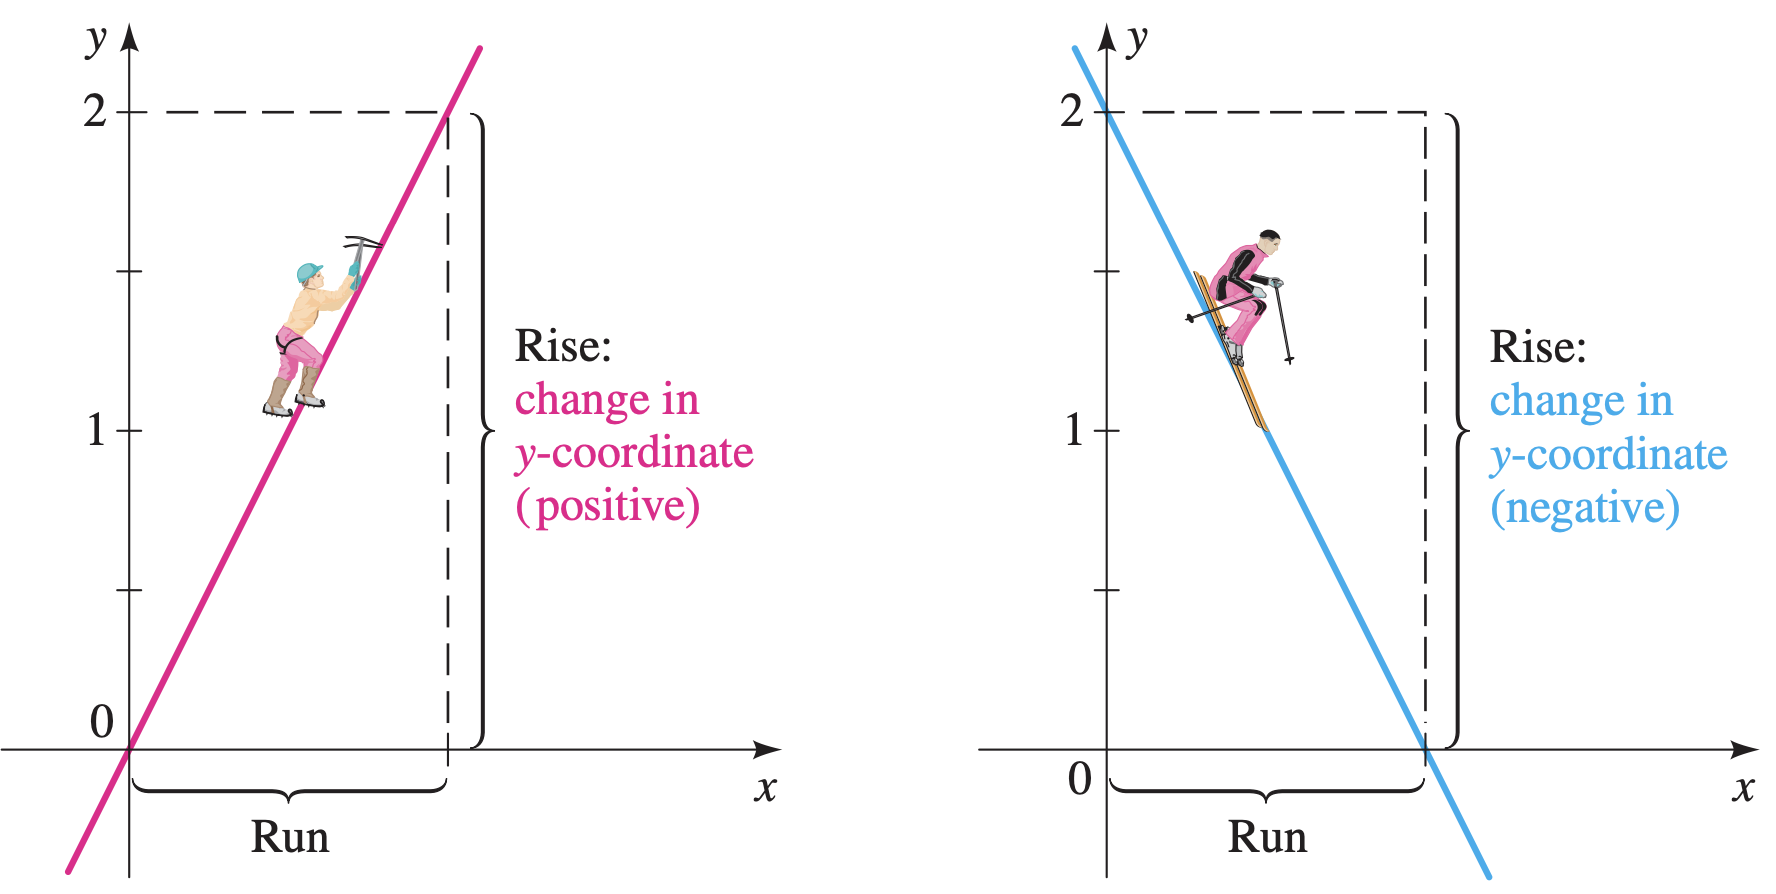
\includegraphics[scale=0.3]{chapter001/figures/fig001}
    \caption{Rise and Run}
    \label{fig:Fig1}
\end{figure}

\newtcolorbox{mybox}[1]{colback=blue!5!white,colframe=blue!75!black,fonttitle=\bfseries,title=#1}
\begin{mybox}{Warning}
The slope is independent of which two points are chosen on the line.
\end{mybox}

\begin{figure}[h]
    \centering
    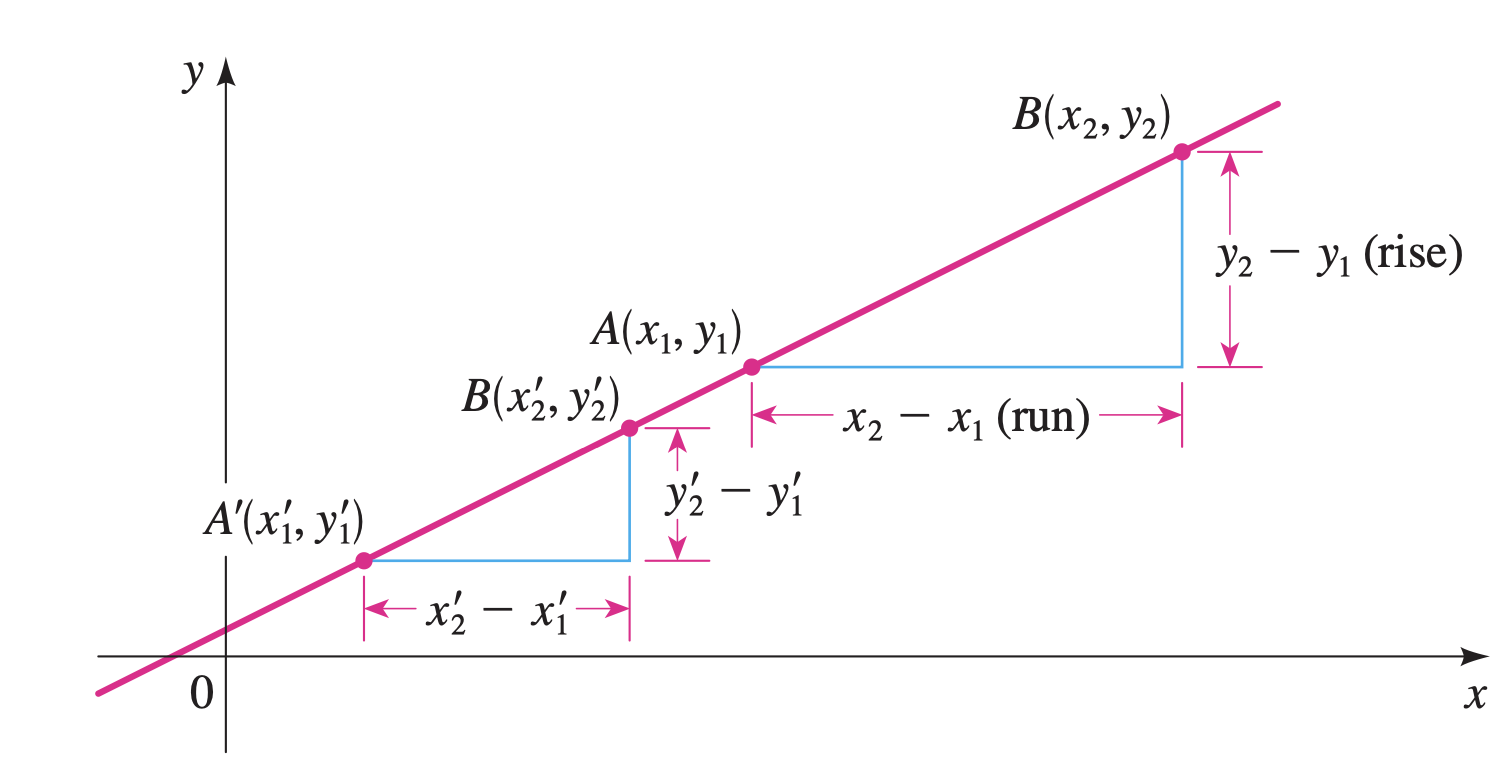
\includegraphics[scale=0.3]{chapter001/figures/fig002}
    \caption{The slope of a vertical line is not define}
    \label{fig:Fig2}
\end{figure}

\begin{figure}[h]
    \centering
    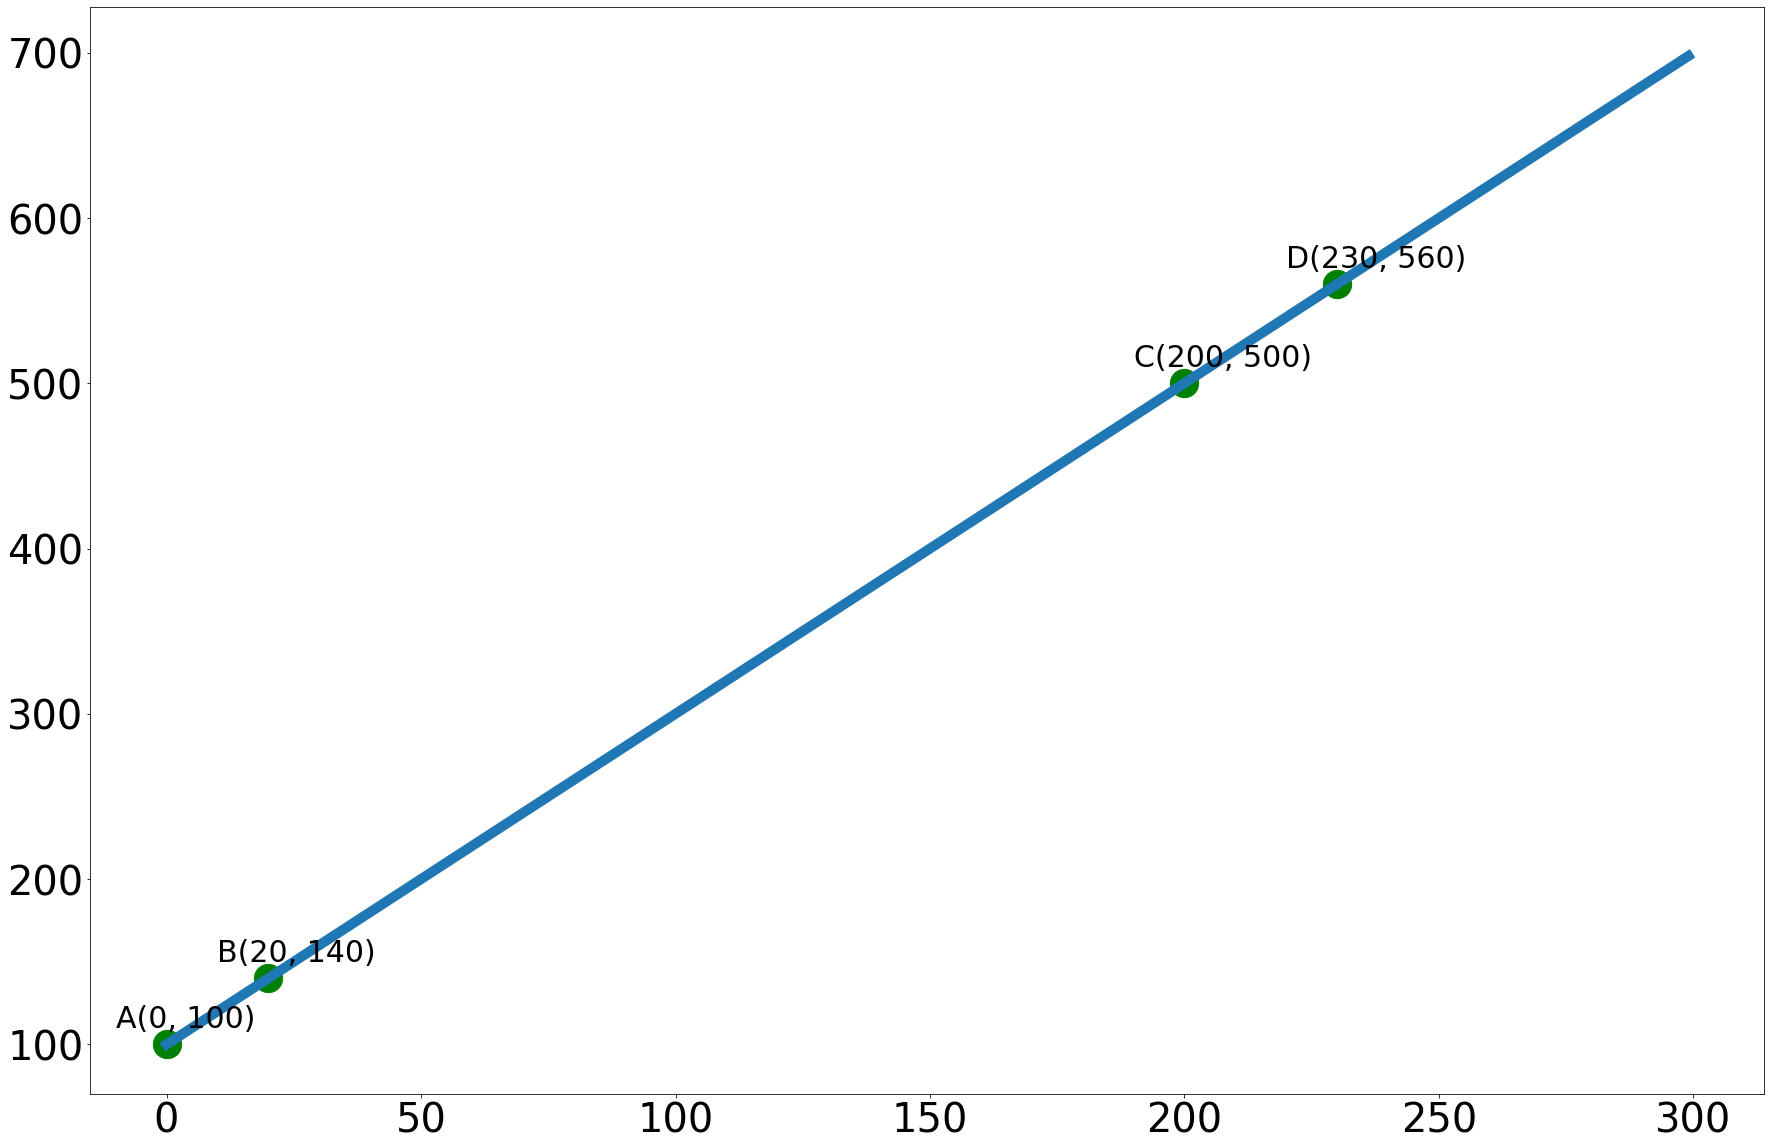
\includegraphics[scale=0.15]{chapter001/figures/fig003}
    \caption{The slope of A and B is the same as C and D}
    \label{fig:Fig3}
\end{figure}

\subsection{Example}
Given 2 lines which are represented by equations $f(x) = 5x + 3$ and $g(x) = 10x + 6$, respectively.

\begin{center}
	\begin{tabular}{ |p{3cm}||p{3cm}|p{3cm}|p{3cm}|}
 		\hline
 		\multicolumn{2}{|c|}{Investigating Steepness Values} \\
 		\hline
 		$f(x) = 5x + 3$ & $g(x) = 10x + 6$\\
 		\hline
 		$x=1, y=8$  & $x=1, y=16$\\
 		$x=2, y=13$ & $x=2, y=26$\\
 		$x=3, y=18$ & $x=3, y=36$\\
 		$x=4, y=23$ & $x=4, y=46$ \\
 		$x=5, y=28$ & $x=5, y=56$\\
 		\hline
	\end{tabular}	
\end{center}

The $g(x)$ is always rise faster than $f(x)$. The steepest lines are those for which the absolute value of the slope is the largest.

\section{Rates of Change} 
\begin{figure}[h]
    \centering
    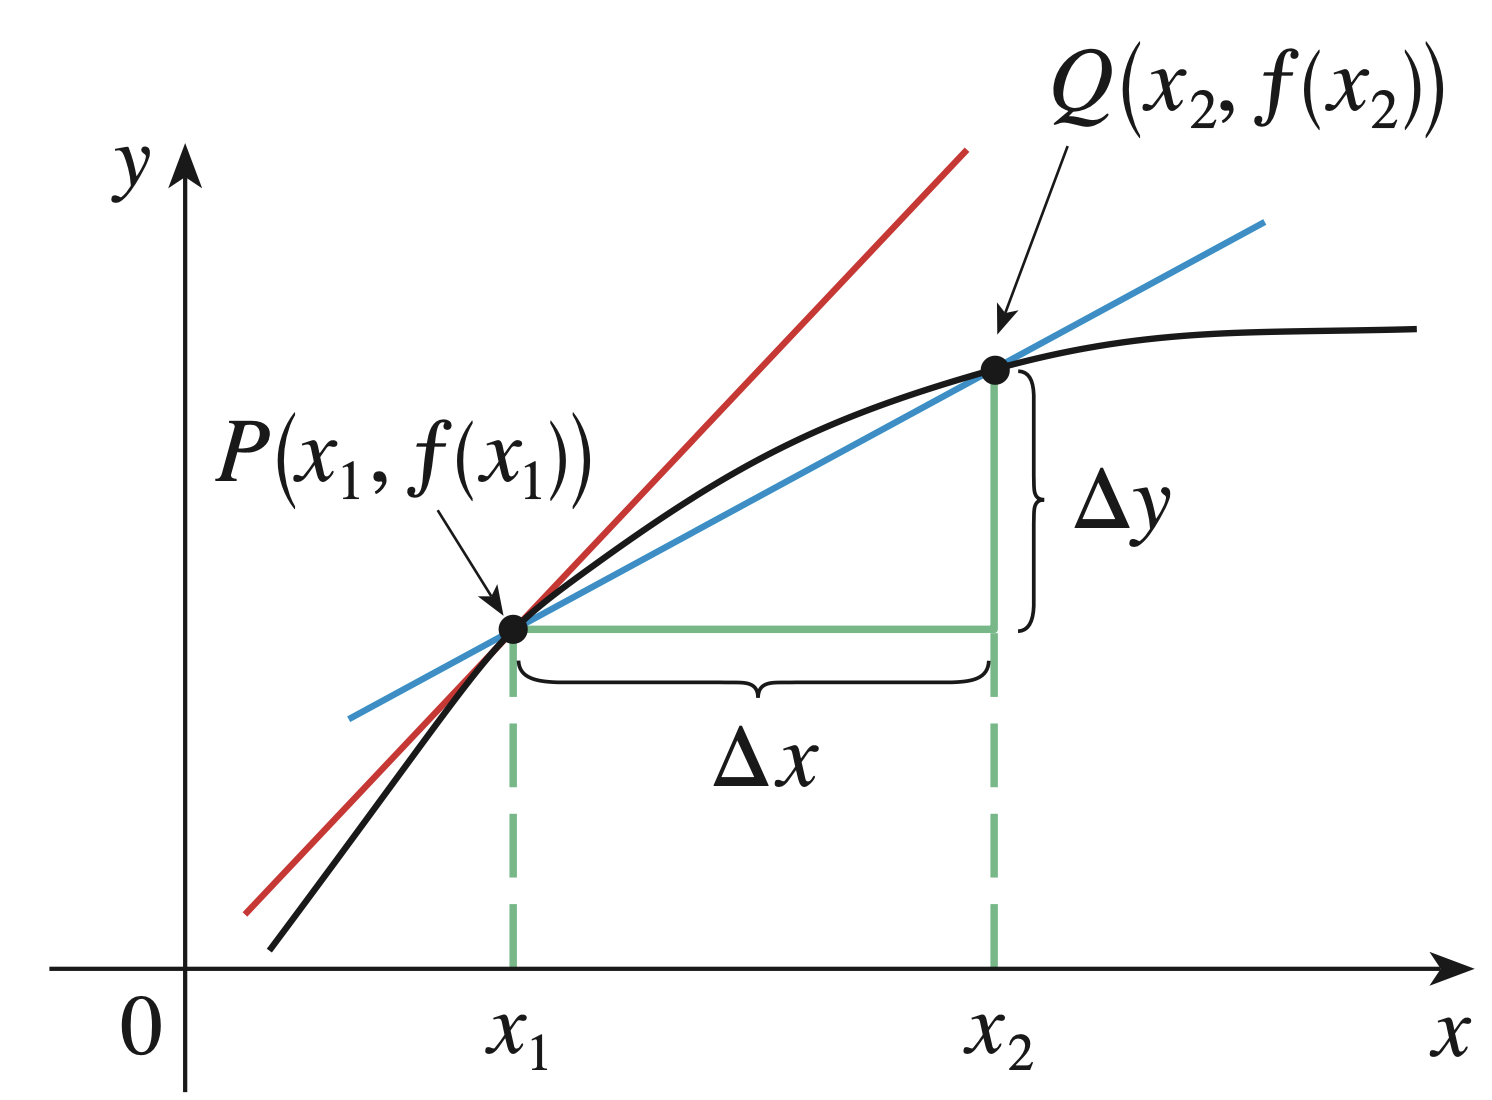
\includegraphics[scale=0.3]{chapter001/figures/fig004}
    \caption{Rates of Change}
    \label{fig:Fig4}
\end{figure}

\begin{flushleft}
\cite{calculus} Given a function $y=f(x)$, if $x$ changes from $x_1$ to $x_2$, then the change in $x$ is $\Delta x = x_2 - x_1$ and the corresponding change in $y$ is $\Delta y = f(x_2) - f(x_1)$.
\end{flushleft}

\begin{flushleft}
The difference quotient

\begin{equation}
\label{eq:2}
\frac{\Delta y}{\Delta x} = \frac{f(x_2) - f(x_1)}{x_2 - x_1}
\end{equation}

is called the \textbf{average rate of change of y with respect to x} over the interval $[x_1, x_2]$ and can be interpreted as the slope of the secant line $PQ$ in Figure \ref{fig:Fig4}

We now consider the average rate of change over smaller and smaller intervals by letting $x_2$ approach $x_1$ and therefore letting $\Delta x$ approach 0.

The limit of these average rates of change is called the (\textbf{instantaneous}) \textbf{rate of change of $y$ with respect to $x$} at $x = x_1$, which is interpreted as the slope of the tangent to the curve $y = f(x)$ at $P(x_1, f(x_1))$
\end{flushleft}

\begin{equation}
\label{eq:3}
instantaneous\ rate\ of\ change = \lim_{\Delta x \to 0} \frac{\Delta y}{\Delta x} = \lim_{x_2 \to x_1} \frac{f(x_2) - f(x_1)}{x_2 - x_1}
\end{equation}

\begin{flushleft}
We recognize this limit as being the derivative $f'(x_1)$.
we know the one interpretation of the derivative $f'(a)$ is as the slope of the tangent line to the curve $y=f(x)$ when $x=a$
\end{flushleft}

\begin{mybox}{Derivative}
The derivative $f'(a)$ is the instantaneous rate of change of $y=f(x)$ with respect to $x$ when $x = a$.
\end{mybox}

\begin{flushleft}
The connection with the first interpretation is that if we sketch the curve $y = f(x)$, then the instantaneous rate of change is the slope of the tangent to this curve at the point where $x = a$.

This means that when the derivative is large, the y-values change rapidly. When the derivative is small, the curve is relatively flat (as at point $Q$) and the y-values changes slowly.
\end{flushleft}

\section{Partial Derivative}
\begin{definition}
If $f$ is a function of two variables, its partial derivatives are the functions $f_x$ and $f_y$ defined by
\end{definition}
\begin{equation}
    \label{eq:7}
    f_x(x, y) = \lim_{\Delta h \to 0} \frac{f(x+h, y)-f(x, y)}{h}
    f_y(x, y) = \lim_{\Delta h \to 0} \frac{f(x, y + h)-f(x, y)}{h}
\end{equation}

\subsection{Example}
If $f(x, y)=x^3+x^2y^3-2y^2$, find $f_x(2,1)$ and $f_y(2,1)$.
\subsubsection{Solution}
$$
    f_x(x, y) = 3x^2 + 2xy^3
$$
and
$$
    f_x(x, y) = 3x^2y^2 - 4y
$$
therefore,
$$
    f_x(2, 1) = 12 + 4 = 16
$$
$$
    f_y(2, 1) = 12 - 4 = 8
$$

\section{Interpretations of Partial Derivatives}

Given an equation $z=f(x, y)$ which represents a surface $S$ (the graph of $f$). If $f(a, b)=c$, then the point $P(a, b, c)$ lies on $S$. As described in the Figure \ref{fig:Fig7}, by fixing $y=b$, we are restricting our attention to the curve $C_1$ in which the vertical plane $y=b$ intersects S. Likewise, the vertical plane $x=a$ intersect $S$ in a curve $C_2$. Both of the curves $C_1$ and $C_2$ pass through the Point $P$.

Note that the curve $C_1$ is the graph of the function $g(x)=f(x, b)$, so the slope of its tangent $T_1$ at $P$ is $g'(a)=f_x(a, b)$. The curve $C_2$ is the graph of the function $G(y)=f(a, y)$, so the slope of its tangent $T_2$ at $P$ is $G'(b)=f_y(a, b)$.

Thus the partial derivatives $f_x(a, b)$ and $f_y(a, b)$ can be interpreted geometrically as the slope of the tangent lines at $P(a, b, c)$ to the traces $C_1$ and $C_2$ of $S$ in the plane $y=b$ and $x=a$.

\subsection{Example}

\cite{calculus} The body mass index (BMI) of a person as

\begin{equation}
    \label{eq:8}
    B(m, h)=\frac{m}{h^2}
\end{equation}

Calculate the partial derivatives of $B$ for a young man with $m=64kg$ and $h=1.68m$ and interpret them.

\subsubsection{Solution}

$$
    \frac{\partial B}{\partial m}(m, h)=\frac{\partial}{\partial m}(\frac{m}{h^2})=\frac{1}{h^2}
$$
so
$$
    \frac{\partial B}{\partial m}(64, 1.68)=\frac{1}{(1.68)^2} \approx 0.35(kg/m^2)/kg
$$
This is the rate at which the man's BMI increases with respect to his weight when he weights $64kg$ and his height is $1.68m$. So if this weight increases by a small amount, one kilogram for instance, and his height remains unchanged, then his BMI will increase from $B(64, 1.68) \approx 22.68$ by about 0.35.

Now we regard $m$ as a constant. The partial derivative with respect to $h$ is 

$$
    \frac{\partial B}{\partial h}(m, h) = \frac{\partial }{\partial h}(\frac{m}{h^2})=m(-\frac{2}{h^3}) = -\frac{2m}{h^3}
$$
so
$$
    \frac{B}{h}(64, 1.68)=-\frac{2 \cdot 64}{(1.68)^3} \approx -27(kg/m^2)/m
$$
This is the rate at which the man's BMI increases with respect to his height when he weights $64kg$ and his height is $1.68m$. If the man is still growing and his weight stays unchanged while his height \textbf{increases} by a small amount, say 1 cm, then his BMI will \textbf{decrease} by about $27(0.01) = 0.27$.


\begin{figure}[h]
    \centering
    \cite{calculus}
    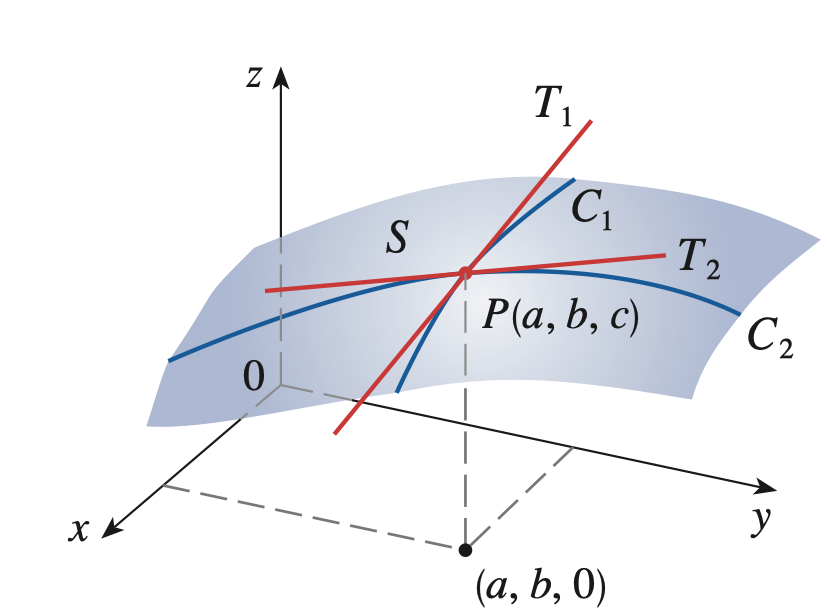
\includegraphics[scale=0.6]{chapter001/figures/fig007}
    \caption{The partial derivatives of $f$ at $(a, b)$ are the slope of the tangents to $C_1$ and $C_2$}
    \label{fig:Fig7}
\end{figure}

\section{The Chain Rule}

\begin{definition}
If $g$ is differentiable at $x$ and $f$ is differentiable at $g(x)$, then the composite function $F=f \circ g$ defined by $F(x)=f(g(x))$ is differentiable at $x$ and $F'$ is given by the product
    \begin{equation}
	   \label{eq:9}
	   F'(x) = f'(g(x)) \cdot g'(x)
    \end{equation}
In Leibniz notation, if $y=f(u)$ and $u=g(x)$ are both differentiable functions, then
    \begin{equation}
	   \label{eq:10}
	   \frac{dy}{dx}=\frac{dy}{du}\frac{du}{dx}
    \end{equation}
\end{definition}

\subsection{Example}

\cite{calculus}, page 202. Differentiate (a) $y=sin(x^2)$ and (b) $y=sin^2x$.

\subsubsection{Solution}
(a) If $y=sin(x^2)$, then the outer function is the sine function and the inner function is the squaring function, so the Chain Rule gives
$$
    \frac{dy}{dx}=\frac{d}{dx}sin(x^2)=2x \cdot cos(x^2)
$$
(b) Note that $sin^2x=(sinx)^2$,
$$
    \frac{dy}{dx}=\frac{d}{dx}(sinx)^2=2 \cdot sinx \cdot cosx
$$

\begin{definition}
Suppose that $z=f(x, y)$ is a differentiable function of $x$ and $y$, where $x=g(t)$ and $y=h(t)$ are both differentiable functions of t. Then z is a differentiable function of $t$ and

    \begin{equation}
        \label{Chain Rule Case 1}
        \frac{dz}{dt}=\frac{\partial f}{\partial x}\frac{\partial x}{\partial t} + \frac{\partial f}{\partial y}\frac{\partial y}{\partial t}
    \end{equation}
\end{definition}

\begin{definition}
    Suppose that $z=f(x, y)$ is a differentiable function of $x$ and $y$, where $x=g(s, t)$ and $y=h(s, t)$ are differentiable functions of $s$ and $t$.
\end{definition}
\noindent
\begin{tabularx}{\linewidth}{@{}XX@{}}
    \begin{equation}
        \label{Chain Rule Case 2}
        \frac{dz}{dt}=\frac{\partial z}{\partial x}\frac{\partial x}{\partial t} + \frac{\partial z}{\partial y}\frac{\partial y}{\partial t}
    \end{equation}
    &
    \begin{equation}
        \label{Chain Rule Case 2}
        \frac{dz}{ds}=\frac{\partial z}{\partial x}\frac{\partial x}{\partial s} + \frac{\partial z}{\partial y}\frac{\partial y}{\partial s}
    \end{equation}
\end{tabularx}

\begin{definition}
    Suppose that $u$ is a differentiable function of the $n$ variables $x_1, x_2, ..., x_n$ and each $x_j$ is a differentiable function of the $m$ variables $t_1, t_2, ..., t_m$. Then $u$ is a function of $t_1, t_2, ..., t_m$ and
    \begin{equation}
        \label{The General Chain Rule}
        \frac{\partial u}{\partial t_i} = \frac{\partial u}{\partial x_1}\frac{\partial x_1}{\partial t_i} + \frac{\partial u}{\partial x_2}\frac{\partial x_2}{\partial t_i} + ...+ \frac{\partial u}{\partial x_n}\frac{\partial x_n}{\partial t_i}
    \end{equation}
    for each $i=1, 2, ..., m$.
\end{definition}

\subsection{Example}
The pressure $P$ (in kilopascals), volume $V$ (in liters), and temperature $T$ (in kelvins) of a mole of an ideal gas are related by equation $PV=8.31T$. Find the rate at which the pressure is changing when the temperature is $300K$ and increasing at a rate of $0.1K/s$ and the volume is $100L$ and increasing at a rate of $0.2L/s$. (Finding the rate change of $P$)(\cite{calculus}, page 1024)

\subsubsection{Solution}
If $t$ represents the time elapsed in seconds, then at the given instant we have $T=300$, $\frac{dT}{dt}=0.1$, $V=100$, $\frac{dV}{dt}=0.2$. Since
$$
    P = 8.31\frac{T}{V}
$$
thus,
$$
    \Rightarrow \frac{\partial P}{\partial T} = \frac{8.31}{V}
$$
and
$$
    \Rightarrow \frac{\partial P}{\partial V}=-\frac{8.31T}{V^2}
$$
Therefore,
\begin{equation}
    \frac{\partial P}{\partial t}=\frac{\partial P}{\partial T}\frac{\partial T}{\partial t} + \frac{\partial P}{\partial V}\frac{\partial V}{\partial t}=\frac{8.31}{V}\frac{\partial T}{\partial t} - \frac{8.31 T}{V^2}\frac{\partial V}{\partial t}=\frac{8.31}{100}(0.1)-\frac{8.31(300)}{100^2}(0.2)=-0.04155
\end{equation}
The pressure is decreasing at a rate of about $0.042 kPa/s$.

\subsection{Example}
If $z=e^x \sin y$, where $x=st^2$ and $y=s^2t$, find $\partial z / \partial s$ and $\partial z / \partial t$.
\subsubsection{Solution}
$$
    \frac{\partial z}{\partial s}=\frac{\partial z}{\partial x}\frac{\partial x}{\partial s} + \frac{\partial z}{\partial y}\frac{\partial y}{\partial s} = (e^x \sin y)(t^2) + (e^x \cos y)(2st)
$$
$$
    \frac{\partial z}{\partial t}=\frac{\partial z}{\partial x}\frac{\partial x}{\partial t} + \frac{\partial z}{\partial y}\frac{\partial y}{\partial t} = (e^x \sin y)(2st) + (e^x \cos y)(s^2)
$$

\subsection{Chain Rules with Computational Graph}
Consider the function (\cite{mml-book})
\begin{equation}
    f(x) = \sqrt{x^2 + e^{x^2}} + cos(x^2 + e^{x^2})
\end{equation}
let

\begin{tabularx}{\linewidth}{@{}XX@{}XX@{}XX@{}}
    $
        a = x^2
    $
    &
    $
        b = e^a
    $
    &
    $
        c = a + b
    $
    &
    $
        d = \sqrt{c}
    $
    &
    $
        e = \cos (c)
    $ 
    &
    $
        f = d + e
    $
\end{tabularx}
Then,

\noindent
\begin{tabularx}{\linewidth}{@{}XX@{}XX@{}}
    $$
        \frac{\partial a}{\partial x} = 2x
    $$
    &
    $$
        \frac{\partial b}{\partial a} = e^a
    $$
    &
    $$
        \frac{\partial c}{\partial a} = 1
    $$
    &
    $$
        \frac{\partial c}{\partial b} = 1
    $$
\end{tabularx}

\begin{tabularx}{\linewidth}{@{}XX@{}XX@{}}
    $$
        \frac{\partial d}{\partial c} = \frac{1}{2\sqrt{c}}
    $$ 
    &
    $$
        \frac{e}{c} = -\sin (c)
    $$
    &
    $$
        \frac{f}{d} = 1
    $$
    &
    $$
        \frac{f}{e} = 1
    $$
\end{tabularx}

We can compute $\partial f / \partial x$ by looking forward from the output and obtain

\noindent
\begin{tabularx}{\linewidth}{@{}XX@{}XX@{}}
    $$
        \frac{\partial f}{\partial c} = \frac{\partial f}{\partial d}\frac{\partial d}{\partial c} + \frac{\partial f}{\partial e}\frac{\partial e}{\partial c}
    $$
    &
    $$
        \frac{\partial f}{\partial b} = \frac{\partial f}{\partial c}\frac{\partial c}{\partial b}
    $$
    &
    $$
        \frac{\partial f}{\partial a} = \frac{\partial f}{\partial b}\frac{\partial b}{\partial a} + \frac{\partial f}{\partial c}\frac{\partial c}{\partial a}
    $$
    &
    $$
        \frac{\partial f}{\partial x} = \frac{\partial f}{\partial a}\frac{\partial a}{\partial x}
    $$
\end{tabularx}

\begin{tabularx}{\linewidth}{@{}XX@{}XX@{}}
    $$
        \frac{\partial f}{\partial c} = 1 \cdot \frac{1}{2\sqrt{c}} + 1 \cdot (- \sin(c))
    $$ 
    &
    $$
        \frac{\partial f}{\partial b} = \frac{\partial f}{\partial c} \cdot 1
    $$
    &
    $$
        \frac{\partial f}{\partial a} = \frac{\partial f}{\partial b}e^a + \frac{\partial f}{\partial c} \cdot 1
    $$
    &
    $$
        \frac{\partial f}{\partial x} = \frac{\partial f}{\partial c} \cdot 2x
    $$
\end{tabularx}

\begin{figure}[h]
    \centering
    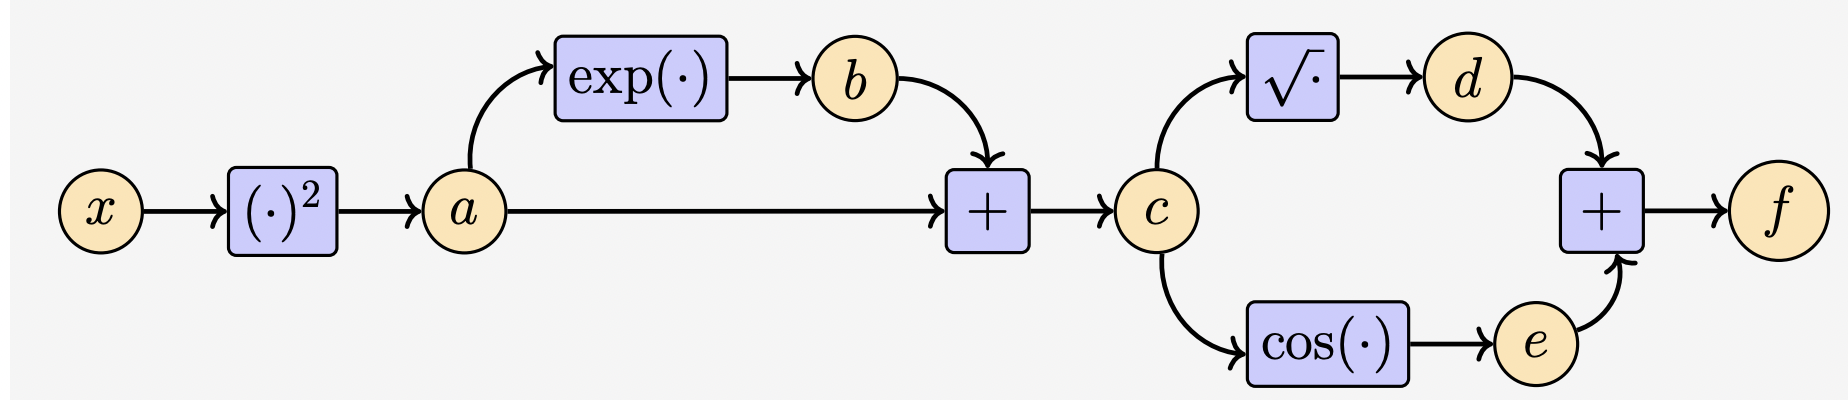
\includegraphics[scale=0.4]{chapter001/figures/fig008}
    \caption{Computational Graph}
    \label{fig:Computational Graph}
\end{figure}


\section{Derivatives of General Exponential Functions}
This content is recommended by \cite{calculus}, page 204.
\begin{theorem}
\begin{equation}
    \label{eq:11}
    \frac{d}{dx}(b^x)=b^x\ln b
\end{equation}    
\end{theorem}

\begin{theorem}
If $n$ is any real number and $u=g(x)$ is differentiable, then
\begin{equation}
    \label{eq:12}
     \frac{d}{dx}(u^n)=nu^{n-1}\frac{du}{dx}
\end{equation}
Alternatively,
\begin{equation}
    \label{eq:12}
     \frac{d}{dx}[(g(x)]^n=n[(g(x)]^{n-1} \cdot g'(x)
\end{equation}    
\end{theorem}

\subsection{Example}
Differentiate $y=(x^3 - 1)^{100}$
\subsubsection{Solution}
Taking $u=g(x)=x^3 - 1$ and $n=100$, we have
$$
    \frac{dx}{dy}=\frac{d}{dx}(x^3 - 1)^{100}=100(x^3 - 1)^{99}\frac{d}{dx}(x^3 - 1)=100(x^3-1)^{99} \cdot 3x^2=300 x^2(x^3-1)^{99}
$$

\subsection{Example}
Differentiate $h(x)=5^{x^2}$

\subsubsection{Solution}
$$
    \frac{dh}{dx}=\frac{d}{dx}(5^{x^2})=5^{x^2} \ln 5 \cdot \frac{d}{dx}(x^2)=2x \cdot 5^{x^2} \ln 5 
$$

\section{Applications in Medicine}

\subsection{Measuring the Rate of Increase of Blood Alcohol Concentration}

Biomedical scientists have studied the chemical and physiological changes in the body that result from alcohol consumption. The reaction in the human body occurs in two stages: a fairly rapid process of absorption and a more gradual one of metabolism. Biomedical scientists have studied the chemical and physiological changes in the body that result from alcohol consumption. The reaction in the human body occurs in two stages: a fairly rapid process of absorption and a more gradual one of metabolism.

Medical researchers measured the blood alcohol concentration (BAC) of eight fasting adult male subjects after rapid consumption of $15 mL$ of ethanol (corresponding to one alcoholic drink).1 The data they obtained were modeled by the concentration function. The graph of C is shown in Figure \ref{fig:Fig5}

\begin{equation}
\label{eq:4}
C(t) = 0.0225te^{-0.0467t}
\end{equation}

where $t$ is measured in minutes after consumption and $C$ is measured in $mg/mL$. How quickly is the BAC increasing after 10 minutes?

\begin{figure}[h]
    \centering
    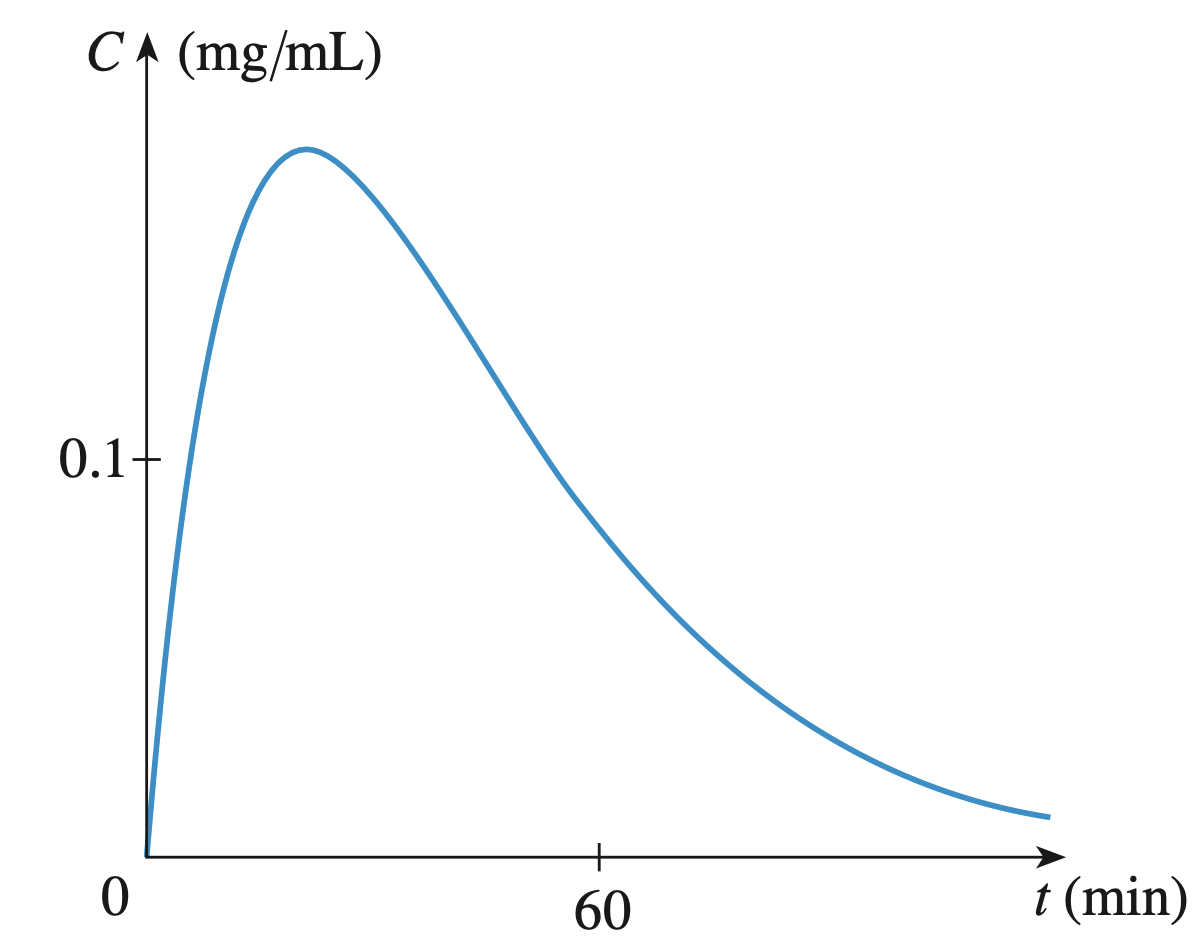
\includegraphics[scale=0.3]{chapter001/figures/fig005}
    \caption{Blood Alcohol Concentration}
    \label{fig:Fig5}
\end{figure}

\begin{center}
	\begin{tabular}{ |p{3cm}||p{3cm}|p{3cm}|p{3cm}|}
 		\hline
 		\multicolumn{2}{|c|}{Investigating Steepness Values} \\
		\hline
 		Time interval & Average rate of change\\
		\hline
 		$10 \leq t \leq 11$    & 0.00703\\
 		$10 \leq t \leq 10.5$  & 0.00727\\
 		$10 \leq t \leq 10.1$  & 0.00747\\
 		$10 \leq t \leq 10.01$ & 0.00751 \\
 		$9 \leq t \leq 10$     & 0.00804\\
 		$9.5 \leq t \leq 10$   & 0.00777\\
 		$9.9 \leq t \leq 10$   & 0.00757\\
 		$9.99 \leq t \leq 10$  & 0.00752\\
 		\hline
	\end{tabular}
\end{center}


\begin{flushleft}
It appears that as we shorten the time period, the average rate of change is becoming closer and closer to a number between 0.00752 and 0.00753 (mg/mL)/min. The instantaneous rate of change at t = 10 is defined to be the limiting value of these average rates of change over shorter and shorter time periods that start or end at t = 10. So we estimate that the BAC increased at a rate of about 0.0075 (mg/mL)/min.

we estimated that the rate of increase of the blood alcohol concentration when $t = 10$ is about 0.0075 (mg/mL)/min. The equation of the curve is \ref{eq:4} which gives $C(10) \approx 0.14105$. So, using the point-slope equation of a line, we get that an approximate equation of the tangent line at $t=10$ is 
\end{flushleft}

\begin{equation}
\label{eq:5}
C - 0.14105 = 0.0075(t - 10)
\Leftrightarrow C = 0.06605 + 0.0075t
\end{equation}

\subsection{Malarial parasites}
The following table, supplied by Andrew Read, shows experimental data involving malarial parasites. The time t is measured in days and N is the number of parasites per micro-liter of blood.

\begin{center}
	\begin{tabular}{ |p{3cm}||p{3cm}|p{3cm}|p{3cm}|}
 		\hline
 		\multicolumn{2}{|c|}{Investigating Steepness Values} \\
 		\hline
 		t & N\\
 		\hline
 		1    & 228\\
 		2    & 2,357\\
 		3    & 12,750\\
 		4    & 26,661\\
 		5    & 372,331\\
 		6    & 2,217,441\\
 		\hline
	\end{tabular}	
\end{center}


\begin{flushleft}
(a) Find the average rates of change of N with respect to t over the intervals [1, 3], [2, 3], [3, 4], and [3, 5].\\
(b) Interpret and estimate the value of the derivative N'(3).
\end{flushleft}

\subsubsection{Solution}

\begin{flushleft}
(a) The average rate of change over [1, 3] is
$$\frac{N(3) - N(1)}{3 - 1} = \frac{12,750 - 228}{2} = 6261 (parasites/\mu L)/day$$
Similar calculations give the average rates of change in the following table:
\end{flushleft}

\begin{center}
	\begin{tabular}{ |p{3cm}||p{3cm}|p{3cm}|p{3cm}|}
 		\hline
 		\multicolumn{2}{|c|}{Investigating Steepness Values} \\
 		\hline
 		Interval & Rate of change\\
 		\hline
 		$[1, 3]$ & 6,261\\
 		$[2, 3]$ & 10,393\\
 		$[3, 4]$ & 13,911\\
 		$[3, 5]$ & 179,791\\
 		\hline
	\end{tabular}	
\end{center}

\begin{flushleft}
(b) The derivative $N'(3)$ means the rate of change of N with respect to $t$ when $t=3$ days.
	$$
		N'(3) = \lim_{\Delta t \to 3} \frac{N(t) - N(3)}{t - 3}
	$$
\end{flushleft}

\subsection{\href{https://www.slideshare.net/ichazalia/derivative-application-in-medical-and-biology}{Growth Rate of Tumor}}

\begin{flushleft}
This example is recommended by \cite{azalia}.\\
There are 3 certain levels of a tumor regarding to its malignancy.
\begin{enumerate}
    \item The first level is benign tumor. It does not invade nearby or spread to other parts of the body.
    \item The second level is premalignant or precancerous tumor which is not yet malignant, but is about to become so.
    \item The last level is malignant tumors. These are cancerous tumors, they tend to become progressively worse, and can potentially result in death.
\end{enumerate}

The rate at which a tumor grows is directly proportional to its volume. Larger tumors grow faster and smaller tumors grow slower.
The volume of a tumor is found by using the exponential growth model which is
	$$
		V(t) = V_0 \cdot e^{kt}
	$$
	where
	
\begin{enumerate}
    \item $V_0$ = initial volume.
    \item e     = exponential growth (2.7182...)
    \item k     = growth constant
    \item t     = time
\end{enumerate}

(a) Find the rate of change of a tumor when its initial volume is $10cm^3$ with a growth constant of 0.075 over a time period of 7 years.\bigbreak
(b) Find the rate of change of a tumor when its initial volume is $2cm^3$ with a growth constant of 0.075 over a time period of 7 years.
\end{flushleft}

\subsubsection{Solution}

The rate of change of a tumor is the derivative of $V(t)$ with respect to $t$
$$
	\frac{\partial v}{\partial t}=\frac{\partial (V_0 \cdot e^{kt})}{\partial t} = k \cdot (V_0 \cdot e^{kt}) = k \cdot (V(t))
$$

(a) 
$$
V(7) = 10 \cdot e^{0.075 \cdot 7} = 16.905(cm^3)
$$
$$
V'(7) = 0.075 \cdot V(7) = 1.267875(cm^3)/year
$$

(b)
$$
V(7) = 2 \cdot e^{0.075 \cdot 7} = 3.3809(cm^3)
$$
$$
V'(7) = 0.075 \cdot V(7) = 0.2535675(cm^3)/year
$$

\begin{mybox}{Question}
What is the tumor growth constant $k$?
\end{mybox}

\subsection{Blood Flow}
This example is based on \cite{calculus} on the page 267.

When we consider the flow of blood through a blood vessel, such as a vein or artery, we can model the shape of the blood vessel by a cylindrical tube with radius R and length l as illustrated in the Figure \ref{fig:Fig6}

\begin{flushleft}
We can calculate the velocity of the blood flow and detect if there are something wrong with the blood pressure or the blood vessel wall.
In this case, we portrait the blood vessel as a cylindrical tube with radius $R$ and length $L$ as illustrated in the Figure \ref{fig:Fig6}
\end{flushleft}

\begin{figure}[h]
    \centering
    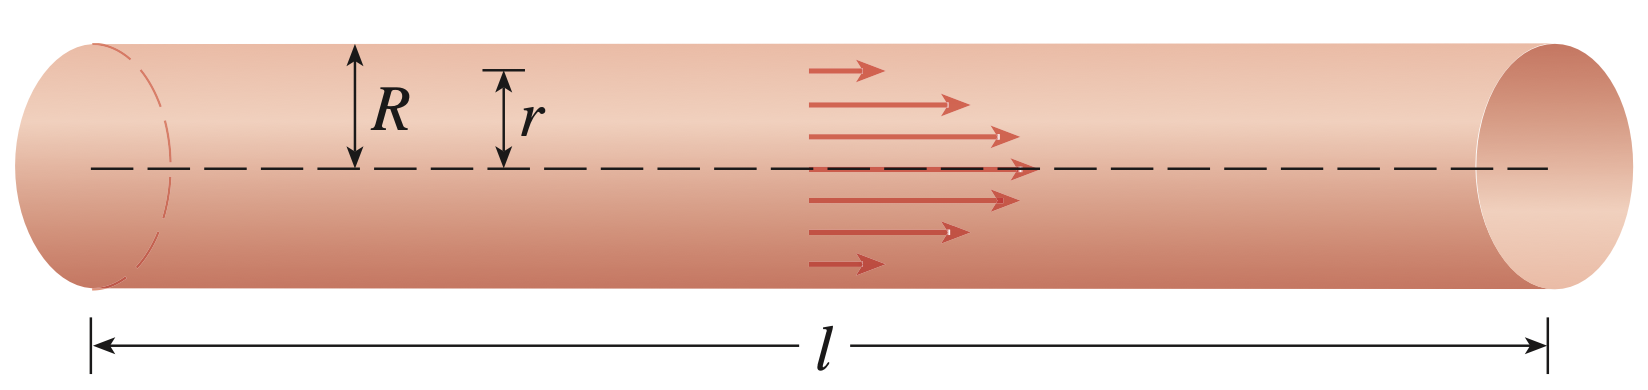
\includegraphics[scale=0.4]{chapter001/figures/fig006}
    \caption{Blood Vessel}
    \label{fig:Fig6}
\end{figure}

\begin{flushleft}
	Because of friction at the walls of the tube, the velocity v of the blood is greatest along the central axis of the tube and decreases as the distance r from the axis increases until v becomes 0 at the wall. The relationship between v and r is given by the law of laminar flow, which was experimentally derived by the French physicist Jean Léonard Marie Poiseuille in 1838. This law states that:
\end{flushleft}

\begin{equation}
	\label{eq:5}
	v = \frac{P}{4 \eta L}(R^2 - r^2)
\end{equation}
where\\
$\eta$ : viscosity of the blood.\\
$P$    : pressure difference between the ends of the blood vessel.\\
$L$    : length of the blood vessel.\\
$R$    : radius of the blood vessel.\\
$r$    : radius of the specific point inside the blood vessel that we want to know

\begin{flushleft}
If $P$ and $l$ are constant, then $v$ is a function of r with domain $[0, R]$. The average rate of change of the velocity as we move from $r=r_1$ outward to $r = r_2$ is given by
\end{flushleft}
$$
\frac{\Delta v}{\Delta r} = \frac{v(r_2) - v(r_1)}{r_2 - r_1}
$$
and if we let $\Delta r \rightarrow 0$, we obtain the velocity gradient, that is

\begin{equation}
	\label{eq:6}
	velocity\ gradient = \lim_{\Delta r \to 0} \frac{\Delta v}{\Delta r} = \frac{dv}{dr}
\end{equation}
Because $P$, $\eta$ and $L$ are constant, then we have
$$
	\frac{dv}{dr} = - \frac{Pr}{2 \eta L}
$$
Given $\eta=0.027$, $R=0.008cm$, $L=2cm$, and $P=4000 \ dynes/cm^2$, which gives
$$
    v = \frac{4000}{4\cdot(0.027)\cdot2} (0.000064 - r^2) \approx 1.85 \cdot 10^4(6.4 \cdot 10^{-5} - r^2)
$$
At $r=0.002cm$ the blood is flowing at a speed of
$$
    v(0.002) \approx 1.85 \cdot 10^4 (64 \cdot 10^{-6} - 4 \cdot 10^{-6}) = 1.11\ cm/s
$$
and the velocity gradient at that point is
$$
    \frac{dv}{dr}=-\frac{4000(0.002)}{2(0.027)2} \approx -74 (cm/s)/cm
$$
To get a feeling for what this statement means, let’s change our units from centimeters to micrometers ($1cm=10000 \mu m$). Then the radius of the artery is $80 \mu m$. The velocity at the center axis is $11,850 \mu m/s$, which decrease to $11,110 \mu m/s$ at a distance of $r=20 \mu m$. The fact that $\frac{dv}{dr}=-74(\mu m/s)/\mu m$ means that, when $r=20\mu m$, the velocity is decreasing at a rate of about $74\mu m/s$ for each micrometer that we proceed away from the center.

\subsection{Economics Cost Function}
Suppose $C(x)$ is the total cost that a company incurs in producing $x$ units of a certain commodity. The function $C$ is called a \textbf{cost function}. If the number of items produced is increased from $x_1$ to $x_2$, then the additional cost is $\Delta C=C(x_2) - C(x_1)$, and the average rate of change of the cost is 
$$
    \frac{\Delta c}{\Delta x}=\frac{C(x_2) - C(x_1)}{x_2 - x_1} = \frac{C(x_1 + \Delta x) - C(x_1)}{\Delta x}
$$
The limit of this quantity as $\Delta x \rightarrow 0$, that is, the instantaneous rate of change of cost with respect to the number of items produced, is called the \textbf{marginal cost} by economist:
$$
    marginal\ cost = \lim_{\Delta x \to 0} \frac{\Delta C}{\Delta x} = \frac{dC}{dx}
$$
Taking $\Delta x = 1$ and $n$ large (so that $\Delta x$ is small compared to $n$), we have
$$
    C'(n) \approx C(n+1) - C(n)
$$
Thus the marginal cost of producing $n$ units is approximately equal to the cost of the producing one more unit [the (n + 1)st unit].\\
It is often appropriate to represent a total cost function by a polynomial
$$
    C(x) = a + bx + cx^2 + dx^3
$$
where a represents the overhead cost (rent, heat, maintenance) and the other terms represent the cost of raw materials, labor, and so on.
For instance, suppose a company has estimated that the cost (in dollars) of producing $x$ items is
$$
    C(x) = 10000 + 5x + 0.01x^2
$$
Then the marginal cost function is
$$
    C'(x) = 5 + 0.02x
$$
The marginal cost at the production level of 500 items is
$$
    C'(500) = 5 + 0.02(500) = \$15/item
$$
This gives the rate at which costs are increasing with respect to the production level when $x=500$ and predicts the cost of the 501st item.\\
The actual cost of producing the 501st item is
$$
    C(501) - C(500) = \$15.01 \approx C'(500)
$$

